%%%%%%%%%%%%%%%%%%%%%%% file template.tex %%%%%%%%%%%%%%%%%%%%%%%%%
%
% This is a general template file for the LaTeX package SVJour3
% for Springer journals.          Springer Heidelberg 2010/09/16
%
% Copy it to a new file with a new name and use it as the basis
% for your article. Delete % signs as needed.
%
% This template includes a few options for different layouts and
% content for various journals. Please consult a previous issue of
% your journal as needed.
%
%%%%%%%%%%%%%%%%%%%%%%%%%%%%%%%%%%%%%%%%%%%%%%%%%%%%%%%%%%%%%%%%%%%

\RequirePackage{fix-cm}

%\documentclass{svjour3}                     % onecolumn (standard format)
%\documentclass[smallcondensed]{svjour3}     % onecolumn (ditto)
%\documentclass[smallextended]{svjour3}       % onecolumn (second format)
\documentclass[twocolumn]{svjour3}          % twocolumn

\smartqed  % flush right qed marks, e.g. at end of proof

\usepackage{graphicx}
%\usepackage{mathptmx}      % use Times fonts if available on your TeX system
%\usepackage{latexsym}

\journalname{J Comput Aided Mol Des}

\begin{document}

\title{USRT: a de novo Ligand Deduplication and Clustering Algorithm using Ultrafast Shape Recognition with Torsions
%\thanks{Grants or other notes about the article that should go on the front page should be placed here. General acknowledgments should be placed at the end of the article.}
}
%\subtitle{Do you have a subtitle?\\ If so, write it here}

%\titlerunning{Short form of title}        % if too long for running head

\author{Hongjian Li \and Kwong-Sak Leung \and Man-Hon Wong}

%\authorrunning{Short form of author list} % if too long for running head

\institute{Hongjian Li \and Kwong-Sak Leung \and Man-Hon Wong\at
Department of Computer Science and Engineering, Chinese University of Hong Kong, Shatin, New Territories, Hong Kong\\
\email{hjli@cse.cuhk.edu.hk}           %  \\
%\emph{Present address:} of F. Author  %  if needed
%\and
%S. Author \at
%second address
}

\date{Received: date / Accepted: date}
% The correct dates will be entered by the editor

\maketitle

\begin{abstract}

We present the first,
ultrafast
can combine with other USR variants, e.g. USRCAT.

\keywords{de novo ligand design \and deduplication \and clustering \and shape recognition}
% \PACS{PACS code1 \and PACS code2 \and more}
% \subclass{MSC code1 \and MSC code2 \and more} % mathematical subject classification numbers
\end{abstract}

\section{Introduction}
\label{intro}

Given a target protein, hundreds of thousands of ligands are usually docked to find out which one has the highest binding affinity. This method is known as virtual screening. However, the entire drug-like space may contain as many as 10 to the power of 100 molecules, so it is impossible to dock all the available ligands. The de novo ligand design strategy is emerging as a complementary method.

$10^{60}$ drug-like molecules \cite{1104} % Review LEA3D paper

AutoGrow \cite{466}, AutoGrow 3.0 \cite{1354}, iSyn \cite{1381}. They use genetic algorithm. Operators include, mutation, addition, crossover, cutting, selection, etc. Goal is to design ligands that have higher binding affinities. Typical method is to grow an initial scaffold by adding fragments. Any of these types of operators could possibly lead to the generation of duplicate ligands.

In the GA operators, duplicate ligands are occasionally generated. Cumulate generation by generation, and getting sereve. Elitism and fitness proportion in GA not work. Illustrate with two figures, one from iSynMCB, one from crossover (same moieties from different parent ligands, resulting from random mixing, Swap the chemical moieties of known ligands. Link the scaffold and fragment through their respective linker hydrogen atoms).

Selection operator done by iSyn externally calls idock \cite{1153} to evaluate the binding affinity of a population of de novo ligands. It is particularly challenging to tell if two ligands are duplicate when they are in significantly different conformations after being docked against the protein (the selection process) (Figure \ref{fig:MRV}).

\begin{figure*}
\minipage{0.5\textwidth}
\centering
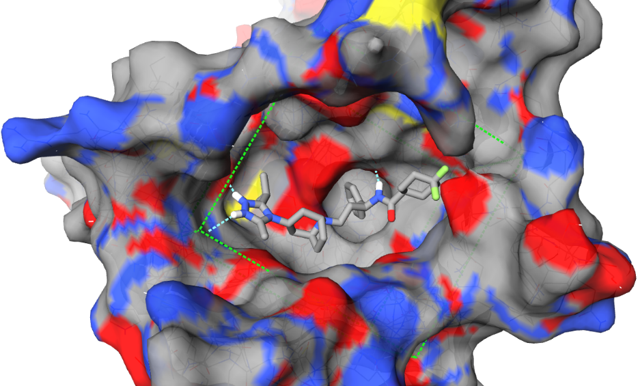
\includegraphics[width=1.36\textwidth,natwidth=638,natheight=386]{../usrt/MRV0.png}
\endminipage
\minipage{0.5\textwidth}
\centering
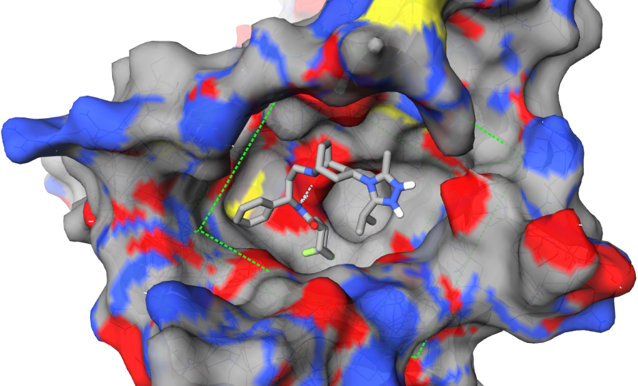
\includegraphics[width=1.36\textwidth,natwidth=638,natheight=386]{../usrt/MRV1.png}
\endminipage
\caption{Two docked poses of the marketed HIV drug maraviroc in complex with the human CCR5 chemokine receptor (PDB ID: 4MBS). The protein is rendered in molecular surface representation. The ligand is rendered in stick representation. The binding cavity on the protein surface is depicted by a green cubic box. The putative intermolecular hydrogen bonds are shown as cyan dashed lines. The ligand poses were generated by idock \cite{1153} and the figure was rendered by iview \cite{1366}.}
\label{fig:MRV}
\end{figure*}

Alignment based methods. Molecular superposition. Precise geometric comparison. Computationally expensive. Similarity score is calculated as the volume overlap.

In iSyn \cite{1381}, we used USR \cite{1379,1280}. Much faster, USR finds its applications in retrospective \cite{1332} and prospective \cite{1380} virtual screening. USR is independent of position and orientation, but is dependent on torsions.

USR variants include USR + MACCS \cite{1333}, Chirality \cite{1334,1335}, lipophilicity into ElectroShape \cite{1337,1338}, USRCAT \cite{1331}. The above variants cannot address the duplication issue. One can use ensemble methods like comparing mwt, nha in addition to USR. These are coarse.

We present USRT, the first algorithm.

In the following sections, we describe USR and USRT, their execution time.

\section{Methods}
\label{sec:methods}

This section introduces USR, USRT.

\subsection{USR: Ultrafast Shape Recognition}
\label{sec:usr}

USR \cite{1379}

Four reference points, ctd: molecular centroid, cst: closest atom to ctd, fct: farthest atom to ctd, ftf: farthest atom to fct. Compute distances. Moments of these distances have semantics. For instance, the 1st, 2nd, 3rd moments of ctd capture the size, variance, skewness of the ligand, respectively. Applicable to different number of atoms. Dimension reduction: any ligand structure is mapped to a point in a 12 dimensional space.

Dissimilarity transformed into a normalized similarity score. (Eq \ref{eqn:usr}) Inverse monotonic function can do.

\begin{equation}
S_{qi}=\frac{1}{1+\frac{1}{12}\sum_{l=1}^{12}|M_l^q-M_l^i|}
\label{eqn:usr}
\end{equation}

Extensible: reference points, moments

\subsection{USRT: Ultrafast Shape Recognition with Torsions}
\label{sec:usrt}

PDBQT format, used by AutoDock series \cite{597,596}, Vina \cite{595}, idock \cite{1153}, QVina \cite{1193}. Explain the PDBQT specification.

Figure \ref{fig:t27} shows two conformations with different torsions. This is a rotatable bond. This branch can rotate along the rotatable bond and flip to the right hand side. A torsion is the rotating angle, so it is in the range of –π to π. 

\begin{figure*}
%\includegraphics[width=\textwidth]{example.png}
\caption{Figure with T27 and T27 with two torsions. T27 is still too complicated. Use half of T27.}
\label{fig:t27}
\end{figure*}

Reference atom is chosen to be the atom connecting to the parent frame. It is BRANCH X Y (Figure \ref{fig:PDBQT}), and is often the first of the current frame. For the ROOT frame, it is the first.

\begin{figure*}
%\includegraphics[width=\textwidth]{example.png}
\caption{Figure of PDBQT lines in Notepad++}
\label{fig:PDBQT}
\end{figure*}

Once a reference atom is determined, the next is to compute inter-atom distances and their 1st, 2nd, 3rd moments.

Frames with less than 2 heavy atoms are ignored.

\section{Results}

\begin{table}
\caption{USRT output feature vector of the nine poses of the same ligand}
\label{tab:1}
\begin{tabular}{rrr}
\hline\noalign{\smallskip}
pose & element 1 & element 2\\
\noalign{\smallskip}\hline\noalign{\smallskip}
1 & 0.2332 & 0.6982\\
2 & 0.2332 & 0.6982\\
\noalign{\smallskip}\hline
\end{tabular}
\end{table}

\subsection{Execution Time Comparison}

USR was claimed to be three orders of magnitude faster than ESshape3D. USR is 1,546 and 2,038 times faster than ESshape3D and Shape Signatures. USR is 14,238 times faster than ROCS, the fastest alignment-based method.

\section{Discussion}

USR has advantages in being independent of position and orientation.

USRT inherits advantages from USR, and is also independent of torsions, which are introduced by flexible ligand docking.

Output is a feature vector, which maps to a point in a high dimensional space. All existing clustering algorithms can be utilized.

Software availability.

Emphasize computational efficiency, 3 orders of magnitude faster than ESshape3D, and applicable to large-scale ligand database like istar \cite{1362}, which has collected 23 million ligands from ZINC \cite{532,1178}.

The current version of USRT has some constraints: known ROOT frame, in-frame atom types, connector atom types. We will address the above limitations in future research.

\section{Availability}

USRT is free and open source under Apache License 2.0. It is available at https://github.com/HongjianLi/usrt and written in C++11. Precompiled executables for 64bit Linux/Windows and examples are provided.

\section{Conclusion}

We have developed USRT (Ultrafast Shape Recognition with Torsions), the first algorithm that can distinguish ligands with different torsions. USRT is computationally very fast, independent of torsions, compatible with USRCAT and other USR variants.

USRT is a general method that can be applied to various drug design applications, including de novo ligand deduplication and clustering.

\section{Author Contributions}

H.L. designed the study, implemented the software, ran the experiments, and wrote the manuscript. All authors discussed results and commented on the manuscript.

\begin{acknowledgements}

This work was supported by the Direct Grant from the Chinese University of Hong Kong and the GRF Grant (Project No. 2150764) from the Research Grants Council of Hong Kong SAR.

\end{acknowledgements}

%\bibliographystyle{spbasic}      % basic style, author-year citations
%\bibliographystyle{spmpsci}      % mathematics and physical sciences
\bibliographystyle{spphys}       % APS-like style for physics
\bibliography{../refworks}   % name your BibTeX data base

\end{document}

%Journal of Computer-Aided Molecular Design 3.172
%Chemical Biology & Drug Design 2.469 
%Molecular Informatics 2.338
%Journal of Molecular Graphics and Modelling 2.325
%IEEE-ACM Transactions on Computational Biology and Bioinformatics 1.616

%Suggested reviewers
%John J. Irwin, UCSF, jir322@gmail.com
%Jacob Durrant, UCSD, jdurrant@ucsd.edu
%Adrian Schreyer, Department of Biochemistry, University of Cambridge, UK, adrian@schreyer.me
%Matthew R. Reynolds, AIDS Vaccine Research Laboratory, 555 Science Dr., Madison, Wisconsin 53711, mrreynol@wisc.edu
%Masaaki Toyama, Center for chronic viral diseases, Kagoshima University, Kagoshima, Japan, toyama@m2.kufm.kagoshima-u.ac.jp
%Pablo Campomanes, German Research School for Simulation Sciences, p.campomanes@grs-sim.de
%Calvin Yu-Chian Chen, School of Medicine, College of Medicine, China Medical University, Taichung, 540402, Taiwan, ycc929@mit.edu
